\documentclass[a4paper,10pt]{article}

\usepackage[T1]{fontenc}
\usepackage[utf8]{inputenc}
\usepackage{multicol}
\usepackage{upgreek}
\usepackage{color}
\usepackage{amsmath}
\usepackage{amsfonts}
\usepackage{amssymb}
\usepackage{graphicx}
\usepackage[bottom]{footmisc}
\usepackage{multirow}
\usepackage[english]{babel}
\usepackage{float}
\usepackage[hang]{caption}
\usepackage{subfig}
\usepackage{microtype}
\usepackage[pdftex]{hyperref}
\hypersetup{colorlinks=false,pdfborder={0 0 0}}
\usepackage[a4paper]{geometry}


\newcommand{\depth}{9}
\newcommand{\mktit}{
	\thispagestyle{empty}
	\begin{center}
	%\includegraphics[height=0.2\textheight]{./photos/lattice} \\
	\hrulefill \\
	\begin{huge}Contact Potential Difference and Photo Voltage \\ \end{huge} 
	\begin{Large} Comparing the Kelvin Probes \\ \end{Large} \vspace*{0.8cm}

	\begin{large}Timo Bretten  \\\end{large} \vspace*{1.2cm}	
	
	\today \\ \vspace*{0.8cm}
	\begin{LARGE}For the Cahen group\\\end{LARGE}
	
	%\includegraphics[height=0.45\textheight]{./photos/dia}
	\end{center}
	\newpage
	\setcounter{page}{2}
}

\newcommand{\sih}{Si--H}
\newcommand{\wfp}{\ensuremath{\upvarphi _{\text{Probe}}}}
\newcommand{\wfs}{\ensuremath{\upvarphi _{\text{Sample}}}}
\newcommand{\cpd}{\text{CPD}}
\newcommand{\McA}{Mc Allister}
\newcommand{\hopg}{HOPG}
\newcommand{\kp}{KP}
\newcommand{\spv}{SPV}
\newcommand{\ie}{i.e.}
\newcommand{\litmin}{\emph{l}/min}
\newcommand{\wf}{WF}

%Centerfloat from Memoire
\makeatletter
\newcommand*{\centerfloat}{%
  \parindent \z@
  \leftskip \z@ \@plus 1fil \@minus \textwidth
  \rightskip\leftskip
  \parfillskip \z@skip}
\makeatother

\begin{document}
\mktit

\section{Introduction}
The purpose of this manual is to outline the measurements I did to compare the three Kelvin Probes (\kp{}s) in 618, 301 and 101. The one in 618 measures in ambient, 301 in the glove box ($\rightarrow$ nitrogen atmosphere) and the one inside the Lakeshore in 101 (referred to as the \lq{}\McA{}\rq{} ) can measure in ambient, argon atmosphere \& in vacuum, with temperature dependence. Next to measuring the contact potential difference (\cpd{}), all three \kp{}s can be used for surface potential voltage (\spv{}) measurements by illuminating the sample.\\
A standard reference with known and stable work-function, \hopg{}, is used to calibrate the probe, \ie{} to find the work function of the probe head. To compare the three probes, I used \sih{} as a relatively stable and well understood sample.
\subsection{(Brief-)Theory}
When two (semi-)conductors with dissimilar fermi-levels are electrically connceted from their back-side with a gap between them, charge will flow from the material with the lower work function (\wf{}) to the one with the higher \wf{}~\footnote{The work function is defined as the energy needed to remove an electron from a solid to a point in vacuum immediately outside of it}. Electrons will stop flowing when equilibrium is established. As long as there is a gap between the materials, an electrical field will develop in the gap due to the difference in the local vacuum level across this gap. 
The potential drop across the gap is known as the contact potential difference or \cpd{}. When the work functions are expressed in Electron-Volts, the \cpd{} is directly equal to the difference of the \wf{}s:
\begin{equation}
\label{wf}
	|{\cpd}| \, = \, | \wfp \, - \wfs | \, .
\end{equation}
Here, I use the absolute value because the sign of the \cpd{} is ultimately dependent on how the measurement system, the Kelvin Probe, is set up. The materials then behave as a parallel plate capacitor, where the potential drops over the space between the two samples. In such a capacitor, the potential drop is given by
\begin{equation}
\label{cap}
	V \, = \,  \frac{Q}{C(d)} \, , 
\end{equation}
where $C(d)$, the capacitance, is inversely proportional to the distance between the plates $d$, $Q$ is the charge on the surfaces and $V$ is the potential set by the difference in local vacuum levels.\\
The \cpd{} is measured by mechanically vibrating the probe-head, thus periodically changing the size of the gap. This causes the capacitance to change as well and according to Equation \eqref{cap}, charge will again flow from one material to the other resulting in a steady state alternating current. This DC current is nulled by an external current source with known impedance from which the equivalent DC voltage needed to null the current can be calculated. This voltage is equal and opposite to the \cpd{}. Thus, if \wfp{} is known, \wfs{} can easily be calculated from Equation \eqref{wf}.\\
The work function of a semiconductor (with molecular surface modification) is composed of the electron affinity $\upchi$~\footnote{Difference between vacuum-level and bottom of conductionband}, plus the position of the Fermi level in the semiconductor band-gap $\upzeta$ and a surface-charge dependent band-bending term $BB$. $\upzeta$ in turn is dependent on the doping level of the semiconductor and is approximately given by:\\
\begin{minipage}[c]{0.4\textwidth}
	\begin{equation}
	E_{f,n} \, =  E_i \, - \, kT \ln{\frac{n}{n_i}}
	\end{equation}
\end{minipage}	
\hfill
and
\hfill
\begin{minipage}[c]{0.4\textwidth}
	\begin{equation}
	E_{f,p} \, = E_i \, + \, kT \ln{\frac{p}{p_i}}
	\end{equation}
\end{minipage},\\
for n- and p-type semiconductors respectively. The difference in \cpd{} between illuminated and dark conditions is called the surface photo-voltage or \spv{}. For n-type semiconductors, the \spv{} is negative, for p-type it\rq{}s positive. It is, however, common to report absolute values of \spv{}. 


\section{Procedure}
A fresh \hopg{}-surface is prepared by rubbing adhesive tape onto a piece and tearing it off evenly. The piece is mounted onto a sample-holder and the \cpd{} is measured.\\
n-\sih{} (100) with different resitivities/doping-levels is prepared according to a slightly modified standard cleaning procedure: pieces of suitable size are cut, swiped off with ethyl-acetate and successively sonicated for six minutes each in ethyl-acetate, acetone, methanol and water. The pieces are ashered at 100W with 1\litmin O$_2$ and 1.5\litmin Ar for 3 minutes, rinsed with water, etched in 2\% HF, rinsed with water and ashered again as before. The pieces are etched as before, back-contacts are created by applying InGa-eutectic to a scratched back surface. The piece is mounted onto a sample holder and the \cpd{} is measured for at least two minutes each on three different spots per piece. The time the sample is subjected to ambient after etch and before each measurment is recorded and used in a linear fit \lq{}$\Delta (\cpd{})/\Delta \, t$\rq{} to find the -- arguably somewhat hypothetical -- \cpd{} each spot on each piece had right after the etch.\\
p-\sih{}(100) is prepared as n-\sih{}, but the 2\% HF-etch is replaced by a three minutes etch in 5\% buffered-oxide-etch (BOE), a solution of 10:1 by volume NH$_4$F:HF.\\
Alumina-passivated silicon was used as obtained from Nir, 
Aluminium coated silicon was prepared by Igal: the sample used was moderately doped n-Si (100). The preparation was identical to the one outlined above, excluding the last etch. Thus, 50nm Aluminium was thermally evaporated onto oxide-terminateda silicon. 
%TABLE WITH MATERIAL PROPERTIES AND ANNOTATIONS

\section{Results \& Discussion}
\subsection{Callibration with \hopg{} and general remarks}
\paragraph{General}
The noise peak-to-peak distance is typically on the order of 10 mV, good measurements can be obtained with a signal peak-peak-distance of three times that value. For \hopg{} and \sih{} distances of as high as 90-120 mV can be reached.\\
The work function of freshly cleaved \hopg{} changes with -0.9 to -1.2 mV per minute. The difference in measured \cpd{} between successively cleaved \hopg{} surfaces is of the order of $\sim$10 mV. The difference of the work function of the probe-head on different dates can be greater~\footnote{Someone else -- or I, for that matter -- measured a \cpd{} and touched their sample with the probe...}, up to 100 mV. With good noise-reduction~\footnote{If necessary, turn off lights and air-conditioning in the room} the machine noise level can be brought down to $\pm$10 mV.
\paragraph{\McA{}}
A jump of 20-40 mV can be observed when switching on the weak pump and a similar jump of $\sim$10 mV is often observed when switching on the turbo pump. These jumps are inconsistent in size and direction and can thus best be interpreted as a displacement of the probe head over the sample. The \cpd{} of \hopg{} in the \McA{} is independent of temperature to within 10 mV, measured over the range of 50K to 300K, in steps of 50K, in both directions (cooling down and heating up).
\begin{figure}[h]
\centerfloat
	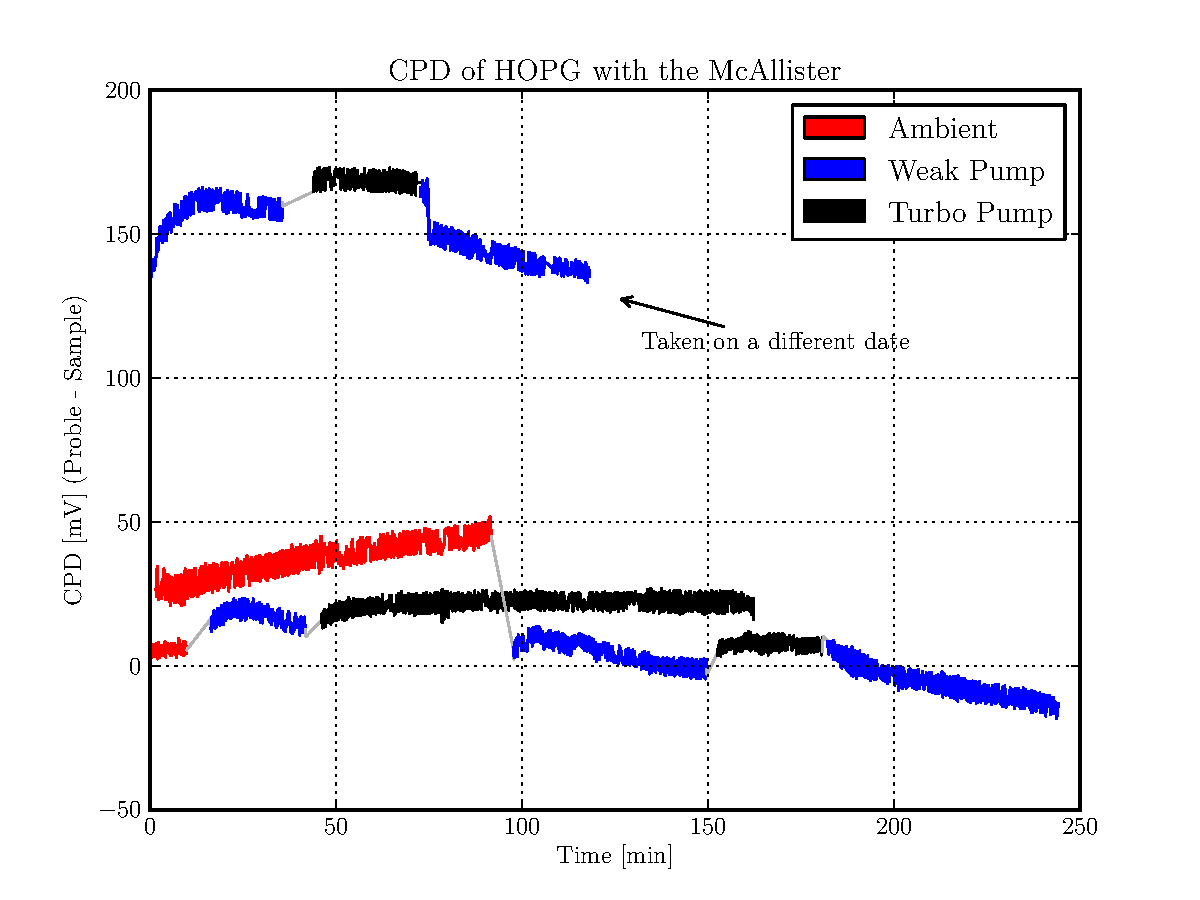
\includegraphics[width=0.75\textwidth]{HOPGMcA}
		\hspace{-0.08\textwidth}
	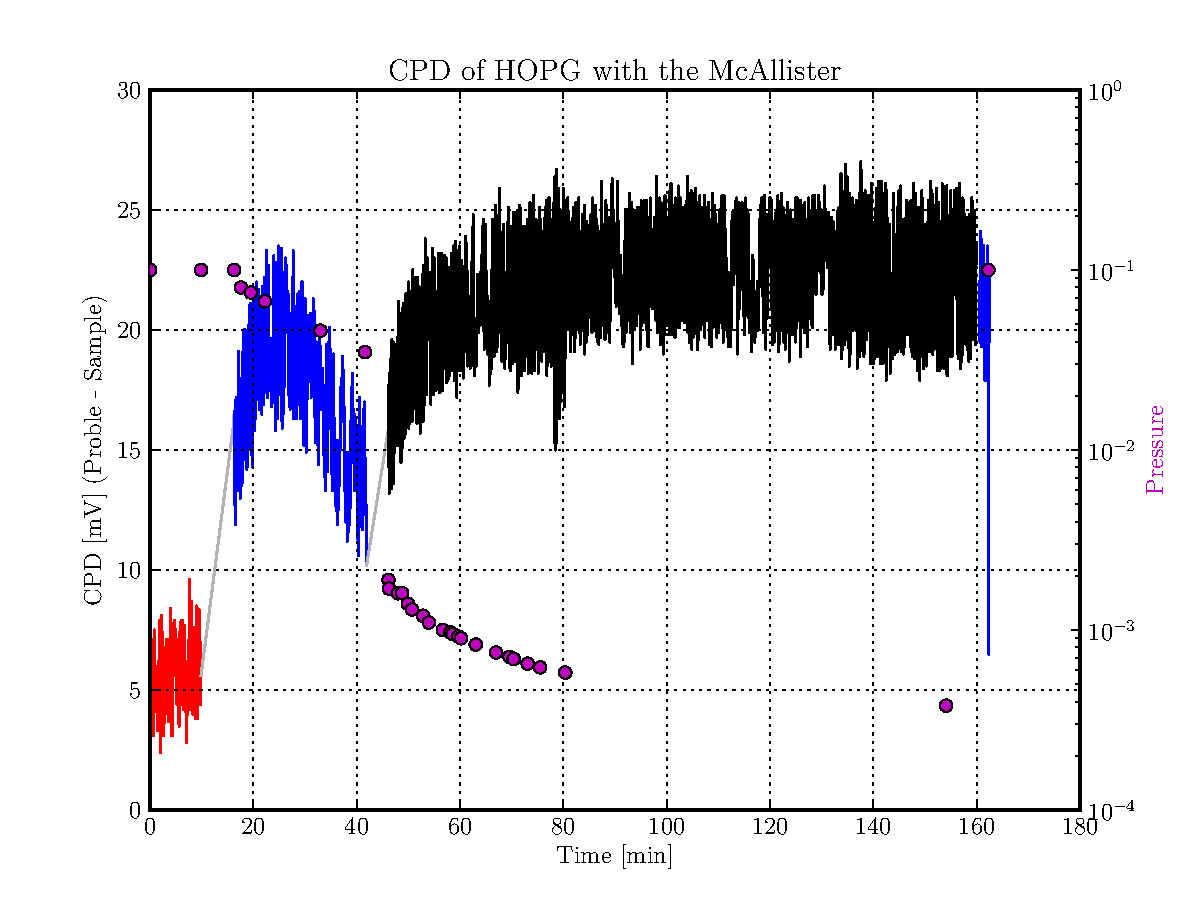
\includegraphics[width=0.75\textwidth]{HOPGMcAPres}
	\caption{\hopg{} measurements in the \McA{}}
		\label{fig:hopgmca}
\end{figure}
\paragraph{Glove box}
The difference in \cpd{} between \hopg{} cleaved inside the glove box and \hopg{} cleaved outside and brought into the box is 60 $\pm$ 30 mV. The work function of \hopg{} when cleaved outside is lower than when cleaved inside, consistent with the observed degradation of \hopg{} in ambient, \ie{} its decrease in \wf{}. Thus, for calibration, \hopg{} has a \wf{} of 4.65 $\pm$ 0.01 eV when cleaved in an inert atmosphere and 4.59 $\pm$ 0.06 eV when cleaved in air.\\

\subsection{Comparison}
\paragraph{n-\sih{}}
The standard deviation of measured \cpd{} between spots of the same piece is comparable to that between pieces, so all obtained values were averaged. The values obtained across the three systems agree very well with each other and in the case of mid- and high-resistivity silicon also with theory, see Figure \ref{fig:nsih}. A three,  instead of only one, minute long HF etch did not influence the \cpd{} obtained for the low resistivity sample. Here, frankly, the wafers were old and the box might have been mislabelled. Another explanation for the deviation from theory might be that the method fails because the surface-reactivity of silicon increases with doping-level. Thus for highly-doped silicon, the linear extrapolation could be more \lq{}hypothetical\rq{} than for the other two conditions. 
\begin{figure}[h]
\label{fig:nsih}
	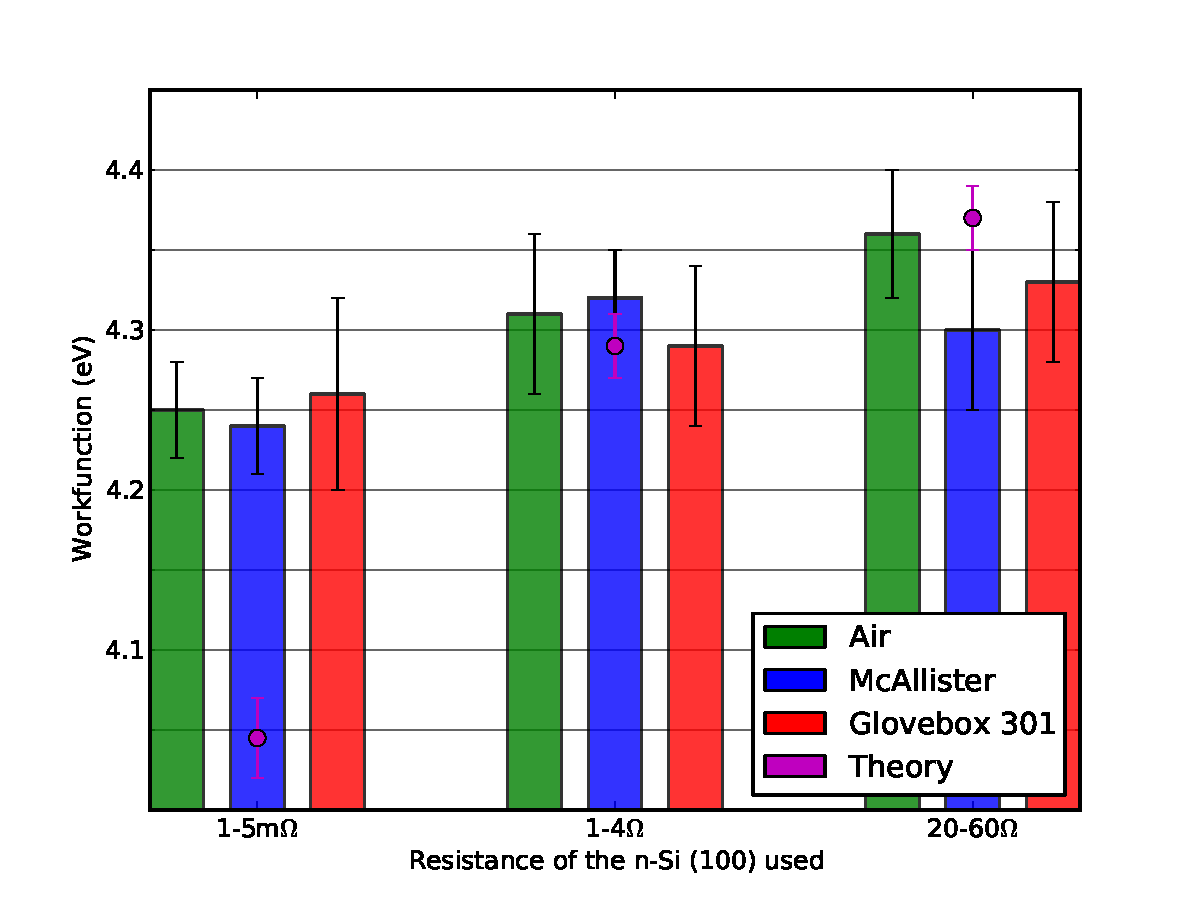
\includegraphics[width=1\textwidth]{Sih}
\caption{Summary of the measured work functions for the n-\sih{} samples used. Indicated errors include deviations in the samples \& the inaccuracy of calibration with \hopg{}.}
	\label{fig:nsih}
\end{figure}

\paragraph{p-\sih{}}
\paragraph{Alumina and aluminium coated silicon}
The \wf{} of alumina passivated silicon was found to be 4.41 eV in 618 and 4.37 eV in the \McA{}. \spv{} was 540 $\pm$ 10 mV in 618 and 520 $\pm$ 10 mV in the \McA{} using the same illumination set-up.\\
The work function of  (hydrophillic) aluminium coated silicon was 4.0 $\pm$ 0.1 eV in 618 and 4.17$\pm$ X eV in the \McA{}. Apart from the mentioned \lq{}jump\rq{}, the \cpd{} did not change when the sample was cooled to 250 K, confer Table XXX. Apparently, no ice forms on the surface. This stroke of luck might be because the sample is not the coolest point in the \McA{}.
\paragraph{\spv{} in the \McA{}}


\section{Conclusion}
\sih{} is a good system to check and compare Kelvin Probes. It is easily prepared and we have great practical knowledge about it.\\
The three \kp{}s in use agree with each other and (mostly) with theory as well. Reliable measurements can be done with each individual probe. If absolute values, \ie{} work functions, are needed, special care has to be taken to calibrate. I advise to calibrate once before measuring and once after, to check if the probe-head has changed during measurement. Temperature dependent \spv{} will soon be a reality, the effect of warmth on \spv{} has to be investigated further.
\end{document}
